\section{Appendix: Additional material}

\subsection{SBM likelihood and prior}
\label{appdx:sbm}

For reference, we provide the likelihoods and priors for the mircocanonical SBM proposed by \citet{Peixoto-Bayesian-Microcanonical}. We have that the graph $A$ is drawn from the SBM:
%
\begin{equation}
	A \sim \textrm{DC-SBM}_{\textrm{MC}}(b, e, k)
\end{equation}
%
With edges placed uniformly at random but respecting the constraints imposed by $b, e$ and $k$. The likelihood calculation for $p(A|k, e, b)$ then reduces to a case of counting configurations that yield the same adjacency matrix, $\Xi (A)$, and dividing by the total number of configurations possible, $\Xi(e)$. This is why this formulation is given the microcanonical moniker. If we consider the half-edges to be distinguishable for a moment, the total number of configurations that satisfy the $e$ constraint is:
%
\begin{equation}
	\Omega(e) = \frac{\prod_{r} e_r !}{\prod_{r,s : r < s} e_{rs}! \cdot \prod_{r} e_{rr}!!}
\end{equation}
%
Where $e_r \coloneqq \sum_{s} e_{rs}$ and $(2m)!! \coloneqq 2^m m!$. Nevertheless, a great number of these configurations yield the same graph $A$. We denote the number of configurations that yield the adjacency matrix $A$ with $\Xi(A)$, which can be computed as:
%
\begin{equation}
	\Xi(A) \coloneqq \frac{\prod_i k_i !}{\prod i,j : i < j A_{ij} ! \prod_i A_{ii} !! }
\end{equation}
%
Note the similarity between the forms of $\Omega(e)$ and $\Xi(A)$ as $e$ is effectively the adjacency matrix of the block-graph. With these defined we can write the overall likelihood:
%
\begin{equation}
	p(A|k,e,b) = \frac{\Xi(A)}{\Omega(e)}
\end{equation}
%
Obviously, this form is only defined if $A$ respects the constraints imposed by $(k,e,b)$ else the likelihood is 0. With the likelihood defined, we move on to the prior. As discussed in the main text, for the FFBM $b$ is an intermediate variable and not a parameter so we are not free to choose a prior for it. Nevertheless, we can borrow the conditional prior proposed by \citet{Peixoto-Bayesian-Microcanonical} for $p(e, k | b)$:
%
\begin{equation}
	p(e, k | b) = p(e | b) p(k| e, b) = \left[ \specialchoose{ \specialchoose{B}{2} }{ E} \right]^{-1} 
	\cdot \left[ \prod_r \frac{\prod_j \eta_j^r !}{n_r! q(e_r, n_r)} \right]
\end{equation}
%
Where $\specialchoose{n}{m}$ is shorthand for $\binom{n+m-1}{m} = \frac{(n+m-1)!}{(n-1)!(m)!}$ which can be thought of as the total number of distinct histograms with $n$ bins under the constraint they sum to $m$. $E = \frac{1}{2} \sum_{r,s} e_{rs}$ is the total number of edges in the graph. Importantly, $E$ is not allowed to vary and so $p(e|b)$ is uniform with respect to $e$. The variable $\eta_j^r$ is introduced to denote the number of vertices in block $r$ that have degree $j$. Formally, $\eta_j^r \coloneqq \sum_{i} \one\left\{b_i = r \right\} \one \left\{k_i = j \right\}$. Furthermore, $q(m, n)$ is the number of different histograms with at most $n$ non-zero bins that sum to $m$. $q(m, n)$ is related to but different from $\specialchoose{n}{m}$. Recall that $e_r \coloneqq \sum_{s} e_{rs}$ is the total number of half edges in block r and $n_r \coloneqq \sum_{i} \one\{b_i = r\}$ is the number of vertices assigned to block $r$. 

The form of these priors were chosen carefully by \citet{Peixoto-Bayesian-Microcanonical} to more closely match the structure of empirical networks than simple uniform priors. We do not repeat his arguments here.

\subsection{Choosing the MALA step-size}
\label{appdx:step-size}

For sampling from the $\theta$-chain of the block membership generator parameters, we employed the Metropolis Adjusted Langevin Algorithm (MALA). At iteration $t$, the proposed sample is generated by:
%
\begin{equation}
	\theta' = \theta^{(t)} - h_t \nabla U(\theta^{(t)}) + \sqrt{2h_t} \cdot \xi
\end{equation}
%
There are two competing objectives when choosing the step-size $h_t$. On the one hand, we want the step-size to be large so that we arrive at a high density region quickly. However, too large a step-size will lead to a lower acceptance ratio and thus inefficient sampling. A solution to this problem would be to slowly decrease the step-size with $t$ - often called simulated annealing. Therefore, we still have a short burn-in time but will not bounce around the mode for large $t$. As well as the trivial constraint for $h_t$ to be strictly positive, we introduce two further constraints as outlined by \citet{Bayesian-SGLD}:
%
\begin{equation}
	\sum_{t=1}^{\infty} h_t = \infty \qquad \textrm{and} \qquad
	\sum_{t=1}^{\infty} h_t^2 < \infty
	\label{eqn:h-constraints}
\end{equation}
%
The first constraint ensures that we have cover sufficient distance to arrive at any arbitrary point in our domain, no matter the starting point. The second constraint ensures that once we converge to the mode rather than simply bouncing around it. \citet{Bayesian-SGLD} propose the following form for a polynomially decaying step-size which we adopt:
%
\begin{equation}
	h_t = \alpha(\beta + t)^{-\gamma}
\end{equation}
%
Where $\alpha, \beta, \gamma$ are hyper-parameters to be chosen. We require $\alpha,\beta > 0$ and $\gamma \in (0.5, 1]$ to satisfy equation \ref{eqn:h-constraints}. To reduce the number of hyperparameters we set these to have values given by the equations \ref{eqn:step-size-params}.
%
\begin{equation}
	\alpha = \frac{250 \cdot s}{N} \qquad \beta = 1000 \qquad \gamma = 0.8
	\label{eqn:step-size-params}
\end{equation}
%
Where $N$ is the number of data-points we are considering and now $s$ is the only free variable which we call the step-size scaling. For approximate methods, we can choose to bypass the MH accept-reject entirely to speed up computation. If this is done, the algorithm is instead called stochastic gradient Langevin diffusion (SGLD) \cite{Bayesian-SGLD}. This speeds up computation at the expense of exactness of the method.

Nevertheless, to choose the value of $s$ we must quantify the trade-off between acceptance ratio and burn-in time. We do this by way of an example with the primary school dataset \cite{schools}. We run the $b$-chain for $T_b = 1,000$ iterations and subsample such that $\Tcal_b$ is computed with $\kappa_b=0.2$ and $\lambda_b=5$. We then use this to run the $\theta$-chain for $T_\theta = 10,000$ iterations. The acceptance ratio -- which we denote $r_\alpha$ -- is easy enough to compute as simply the fraction of proposed moves which we accept. However, to quantify burn-in time we must use a different metric. We can plot the mean of the objective function averaged over all samples as a proxy for burn-in time:
%
\begin{equation}
	\bar{U} \coloneqq \frac{1}{T_\theta} \sum_{t \in [T_\theta]} U\left( \theta^{(t)} \right)
\end{equation}
%
As the chain will equilibrate in the vicinity of a minima in $U(\theta)$, the average over all samples is a rough indicator of the speed of burn-in. This assumes that the random starting point has high $U(\theta)$. The higher the value of $\bar{U}$, the longer the chain took to burn in and reach equilibrium. We plot the acceptance ratio $r_\alpha$ and average objective $\bar{U}$ for $10$ values of the step-size multiplier $s$ logarithmically spaced in the range $(10^{-2}, 10^1)$ on figure \ref{fig:step-size-tradeoff}.
%
\begin{figure}[!h]
	\centering
	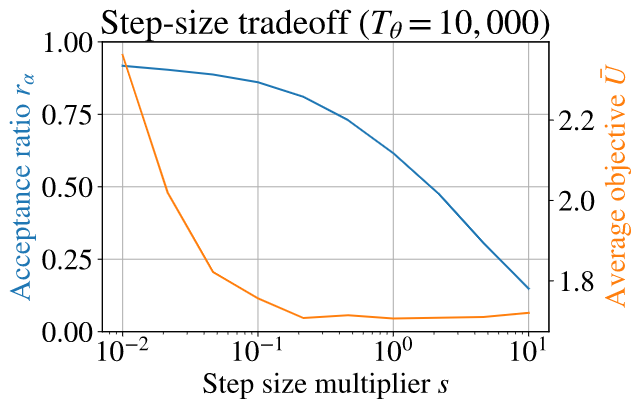
\includegraphics[width=0.6\linewidth]{step-size-tradeoff}
	\caption{Primary school dataset \cite{schools} illustration of step-size tradeoff}
	\label{fig:step-size-tradeoff}
\end{figure}

We see immediately that acceptance ratio $r_\alpha$ steadily decreases with $s$. This is expected as it is unlikely we stay in a high density region of our target distribution if we are making very large steps each time. A low acceptance ratio leads to wasted samples and this inefficiency is obviously undesirable. Nevertheless, $\bar{U}$ decreases with $s$ indicating shorter burn-in times for larger step-sizes. Nevertheless, this effect plateaus for $s>0.2$ for this particular dataset. Therefore, we choose $s=0.2$ as our step-size multiplier for the primary school datasets as this yields the best trade-off between $r_\alpha$ and $\bar{U}$. Indeed, the acceptance ratio is still high for $r_\alpha \approx 0.8$ for $s=0.2$. The step-sizes for the other datasets were chosen following the same argument.

\FloatBarrier
\subsection{Burn-in and thinning}
\label{appdx:burn-in-thinning}

As with any MCMC method, we must deal with the issues presented by burn-in and thinning. We have introduced the notation $\Tcal_b$ and $\Tcal_\theta$ to denote the set of samples we keep from the $b$ and $\theta$ chains respectively. Note that we generate $T_b$ and $T_\theta$ samples total. The burn-in period refers to the time taken for the Markov Chain to converge to the stationary distribution. Sample thinning is necessary to ensure that neighbouring samples satisfy independence. However, as we do not leverage the independence property this is less important in our analysis. We can write the general set $\Tcal_\star$ as:
%
\begin{equation}
	\Tcal_\star = \{T_\star \kappa_\star + i \lambda_\star :  
	0 \leq i \leq \lfloor T_\star(1 - \kappa_\star) / \lambda_\star \rfloor \}
\end{equation}
%
Where the parameter $\kappa_\star \in (0, 1)$ controls our burn-in and $\lambda_\star$ controls our thinning. $\kappa_\star$ can be determined by plotting the log-target (either $S(b^{(t)})$ or $U(\theta^{(t)})$ with respect to the epoch $t$. $\kappa_\star$ is then chosen to encompass the region where the log-target has roughly equilibrated. As we do not leverage sample independence $\lambda_\star$ can be chosen less rigorously. We often just use $\lambda_b=5$ and $\lambda_\theta = 10$.

By way of illustration, we can consider the primary school dataset \cite{schools}. We plot the normalised objective function $U\left( \theta^{(t)} \right) / N$ with respect to MALA iteration on figure \ref{fig:school-U-orginal}. We see that the chain converges to the modal neighbourhood quickly (within about 2000 iterations of a total 10,000). Nevertheless, we pick $\kappa_\theta=0.4 > 0.2$ just to be on the safe-side. $\lambda_\theta=10$ is chosen somewhat arbitrarily as we do not require neighbouring samples to be independent. Nevertheless, this thinning does speed up computation of quantities that require an average over all the retained samples -- as $|\Tcal_\theta| < T_\theta$.
%
\begin{figure}[!h]
	\centering
	\begin{subfigure}[t]{0.4\linewidth}
		\centering
		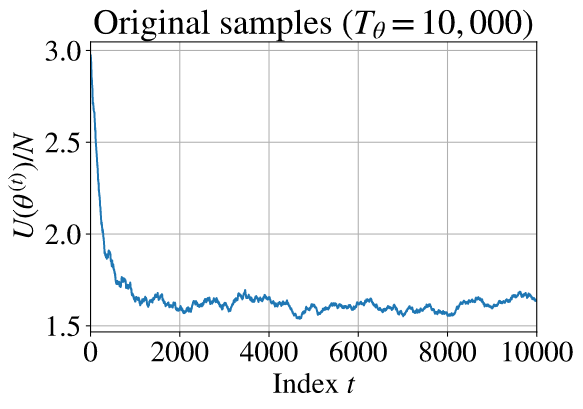
\includegraphics[width=\linewidth]{school-U-original.png}
		\caption{Original samples $t \in [T_\theta]$}
		\label{fig:school-U-orginal}
	\end{subfigure}
	\begin{subfigure}[t]{0.4\linewidth}
		\centering
		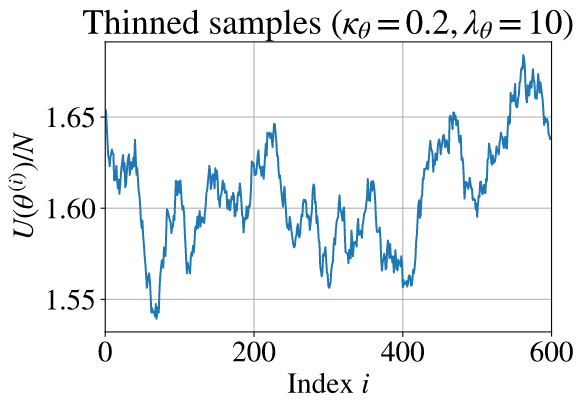
\includegraphics[width=\linewidth]{school-U-thinned.png}
		\caption{Thinned samples $t \in \Tcal_\theta$ indexed by $i$}
		\label{fig:school-U-thinned}
	\end{subfigure}
	\hspace{1cm}
	\caption{Primary school dataset normalised objective function against sample index}
\end{figure}

We see on figure \ref{fig:school-U-thinned} that $U(\theta^{(i)})$ does bounce around a small amount. This is to be expected we are sampling from the posterior rather than converging to the MAP. The variations do appear to be rather long in time-scale but we can live with this as we do not require sample independence.
\FloatBarrier
\subsection{Initializing the b-chain}

For the purposes of our model (the FFBM), the number of blocks $B$ is a constant which must be specified by the data scientist. We could however, allow our choice of $B$ to be influenced by the observed data. This places us in the domain of empirical Bayes, which must be negotiated carefully. Prior beliefs must be determined a priori else they are not prior. However, as the number of blocks only specifies the coarseness of the analysis, it is fine to allow it to vary. Indeed, \citet{peixoto-determine-B} shows that for a fixed average degree the maximum number of detectable blocks scales as $O(\sqrt{N})$ where $N$ is the number of vertices.

If we allow $B$ to vary in the $b$-chain (i.e. new blocks can be created and we permit empty blocks) then it can be run  until a minimum description length (MDL) solution is reached. We take the number of non-empty blocks at the MDL to be our fixed block number $B$ for subsequent analysis. Indeed, it is prudent to start our $b$-chain at this MDL solution as then we can burn-in time is greatly reduced.

\subsection{Dimensionality discussion}
\label{appdx:dimension}

There is a challenge when dealing with vertex-features. Many vertex feature often take only one of several discrete values within a set. For example, with the primary school dataset \cite{schools}, a pupil's school-class can take one of 10 values from \{"1A", "1B", "2A", "2B" \dots "5A", "5B"\}.

It is not immediately obvious how to encode this for the feature-to-block classifier. Although this is technically only a single dimension, we choose to expand the data into a set of 10 binary feature flags $\in \Xcal = \{0, 1\}$. Although only one flag will be set at a time it is the simplest method for representing discrete-valued data. The reason we choose $\Xcal=\{0, 1\}$ and not $\Xcal = \{-1, 1\}$ is that the former allows for simpler analysis of the resulting weight values. When a feature is switched off, it has no impact on the softmax classifier. It is simpler to only model positive relationships. We prefer to say that this block is comprised of the vertices with feature $d$ on rather than this block contains the vertices with feature $d$ switched off. To make this explicit, say we have a feature encoding a pupil's gender: \{"male", "female"\}, we represent this as 2 binary feature flags "male": \{0, 1\} and "female": \{0, 1\}. This approach may seem inefficient but it is vital to ensure we can interpret the resulting parameter distributions.

Nevertheless, this dimensionality expansion means that we cannot include a bias term in our classifier as then the MAP solution is less peaked and our $\theta$-samples will have higher variance. To illustrate this point we need only look at the form of the soft-max classifier with bias vector $\beta$, operating on a vector $x$ which only has feature $d$ turned on such that $x_i = \one\{i = d\}$. Component $j$ of the output is given by:
%
\begin{equation}
	\phi_j(x) = \frac{\exp(w_j^T x + \beta_j)}{\sum_{k=1}^{B} \exp(w_k^T x + \beta_k)} = 
	\frac{\exp(w_{jd} + \beta_j)}{\sum_{k=1}^{B} \exp({w_{kd} + \beta_k})}
	\label{eqn:softmax-bias}
\end{equation}
%
For the case that $x$ can only has one entry $x_d=1$ and the rest are 0, the term $w_{kd} + \beta_k$ is effectively the new weight for component $k$. The bias term $\beta_k$ becomes an unnecessary extra degree of freedom. To illustrate this point, we set $\beta_k=\beta_0 \forall j$. If this is the case then equation \ref{eqn:softmax-bias} can be simplified to:
%
\begin{equation}
	\phi_j(x) = \frac{\exp(\beta_0) \cdot \exp(w_{jd})}{\sum_{k=1}^{B} \exp(\beta_0) \cdot \exp(w_{kd})}
	= \frac{\exp(w_{jd})}{\sum_{k=1}^{B} \exp(w_{kd})}
\end{equation}
%
This expression is independent of $\beta_0$ and so it is free to vary. This is not the whole picture as we also have the prior which introduces a regularisation term which favours weights closer to 0. Nevertheless, for mutually exclusive binary feature flags, the bias term does not add to the expressiveness of the model and only serves to complicate analysis. We therefore remove the bias term from the Softmax classifier. Even for data comprised of several such features (e.g. school class and data) we prefer to discard the bias term. The bias term only serves to decrease the loss function by leveraging information about the size of each detected block and not feature information. We do not wish to be overly confident in our model predictions when such prediction is influenced by block size and not feature information. Indeed, the approach was initially developed with a bias term but we found its removal yielded more reliable and reproducible results. 